\thispagestyle{plain}
\subsection{Franke function}
\noindent In the first part of this project the Franke function \eqref{franke_func} was used as data to analyse.
%
\begin{align} \label{franke_func}
\begin{split}
    f(x,y) &= \frac{3}{4} \, exp\left(- \frac{(9x-2)^2}{4} - \frac{(9y-2)^2}{4}\right) \\
    &+ \frac{3}{4}\, exp\left( - \frac{(9x +1)^2}{49} - \frac{(9y+1)}{10}\right) \\
    &+ \frac{1}{2}\, exp\left( -\frac{(9x-7)^2}{4} - \frac{(9y-3)^2}{4}\right) \\
    &- \frac{1}{5} exp \left( - (9x -4)^2 - (9y-7)^2\right) 
\end{split}
\end{align}
A graphic representation is shown in figure \ref{fig:franke_3d}
\begin{figure}[h]\label{fig:franke_3d}
	\centering
	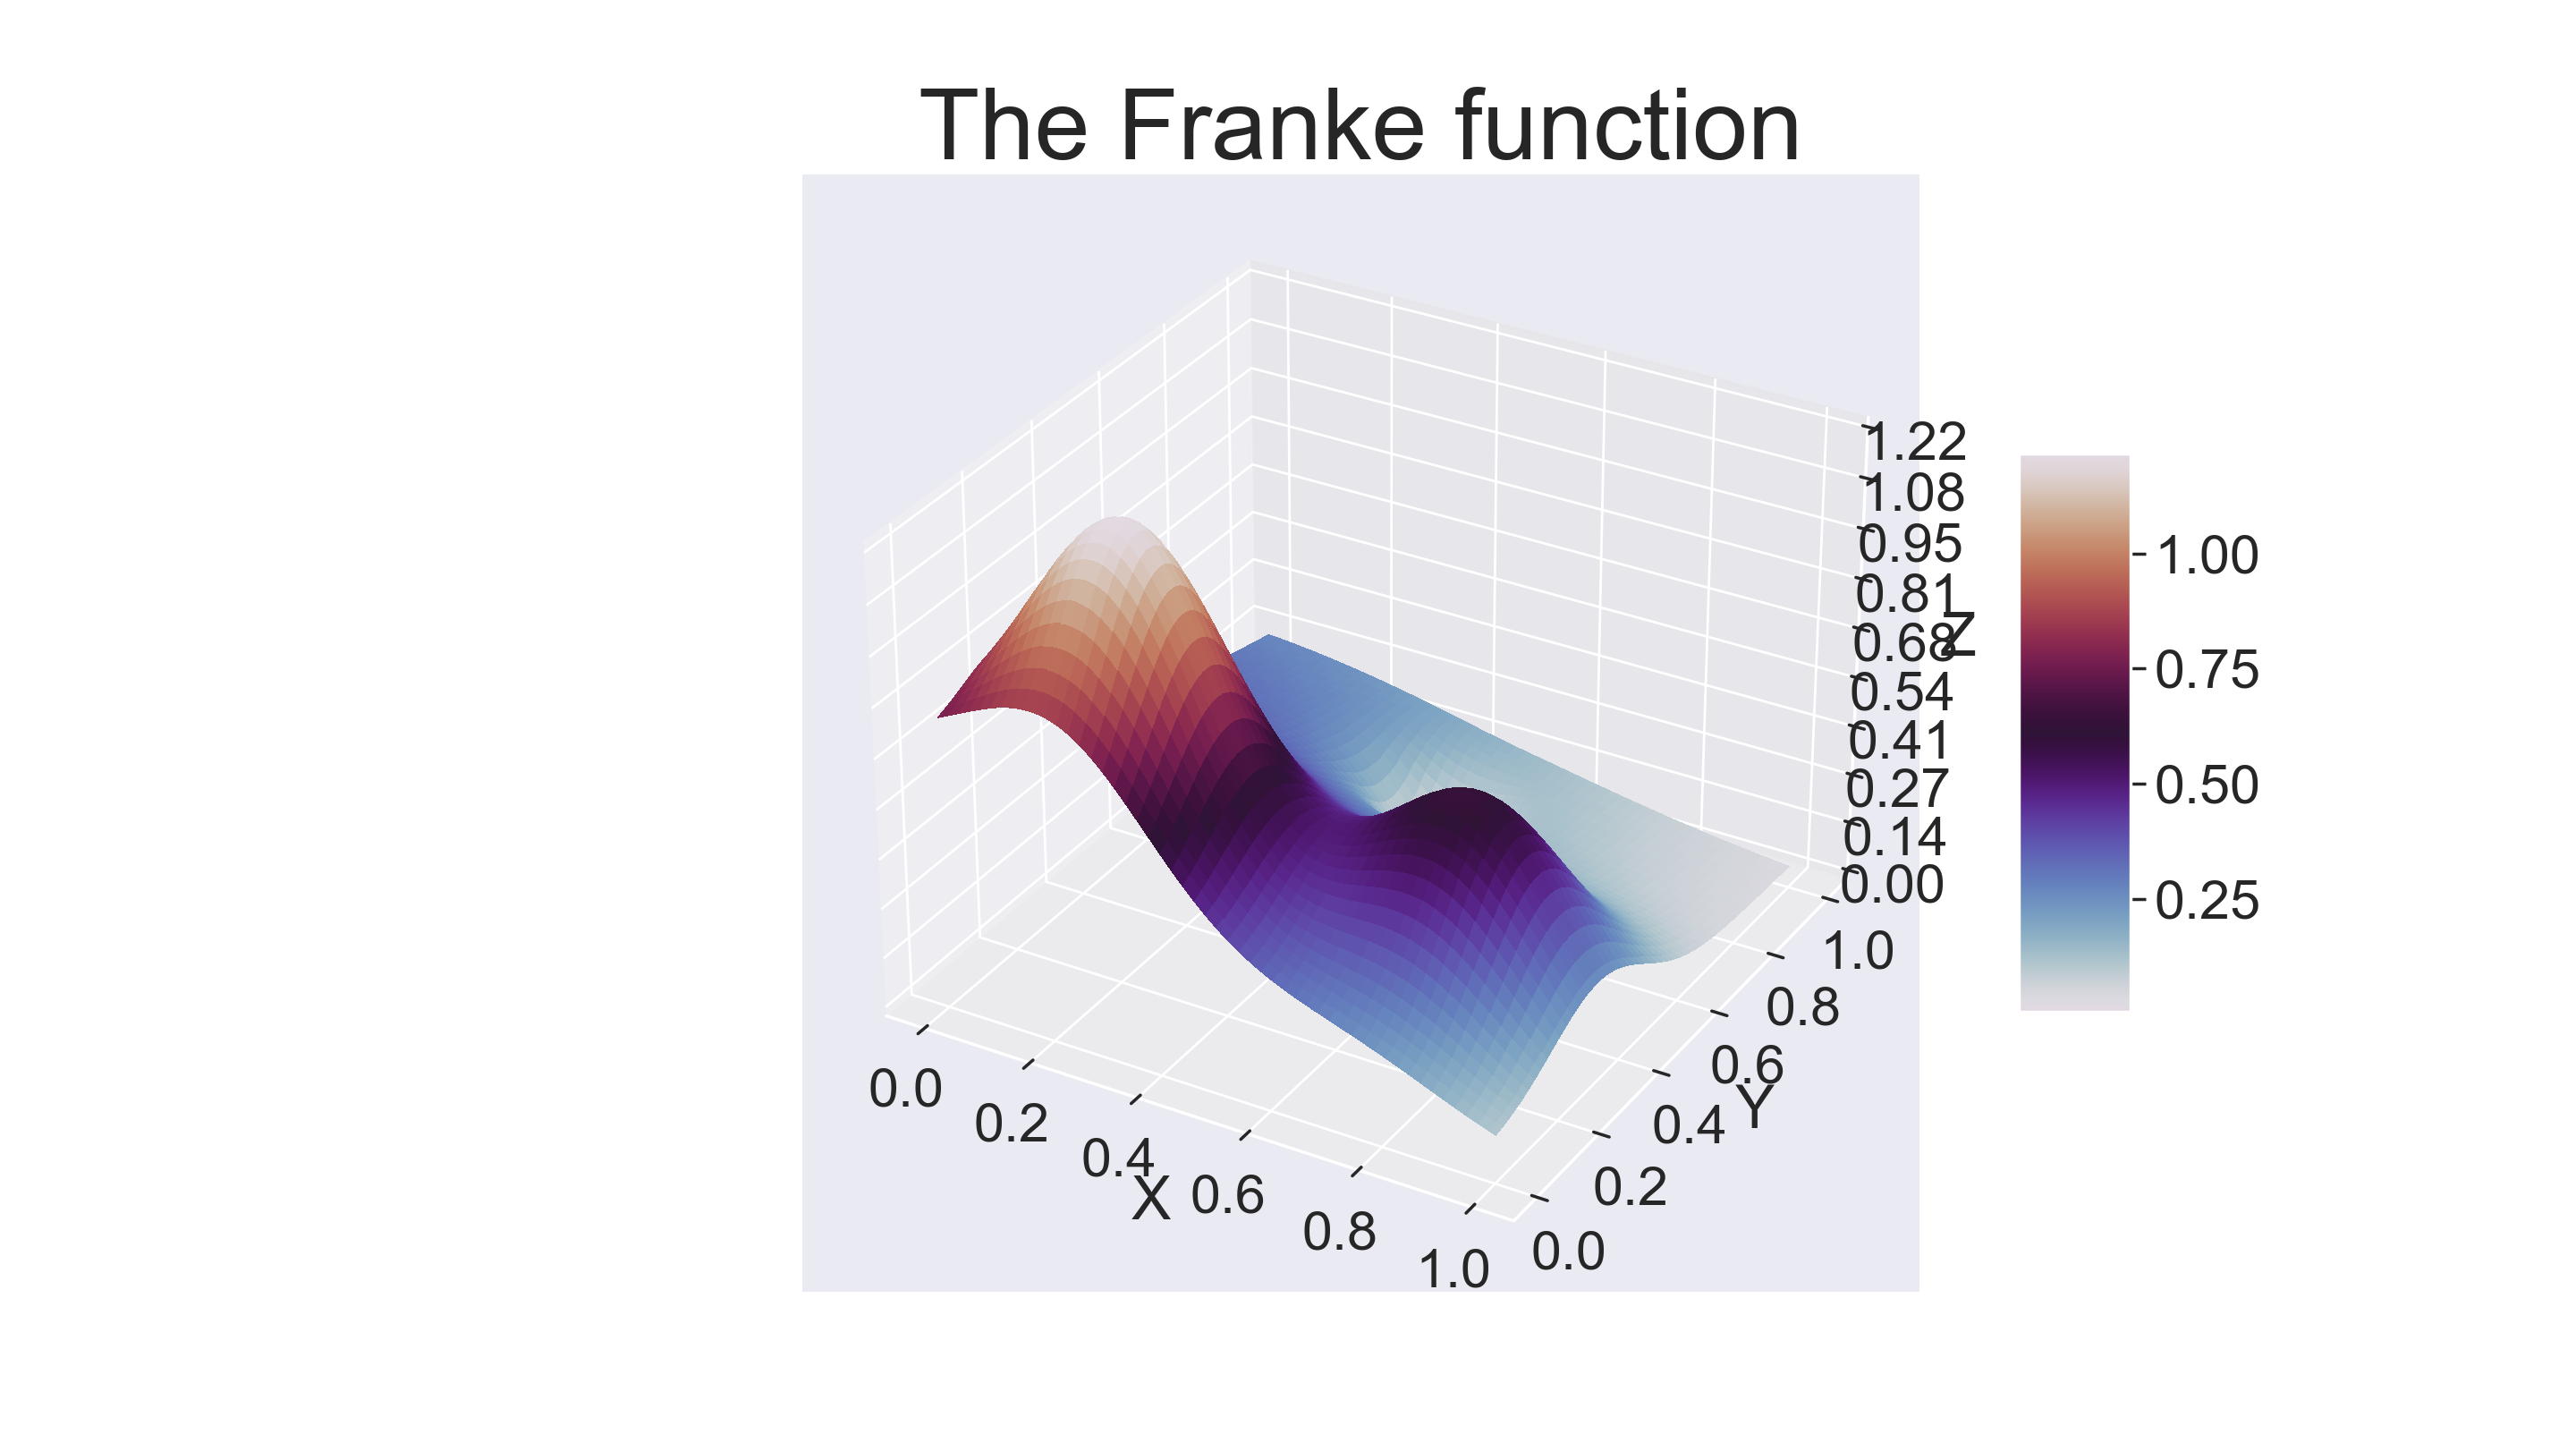
\includegraphics[width=\linewidth]{images/Figure_1.png}
	\caption{\centering A plot of the Franke function }
\end{figure}
%
The number of data points created of the Franke function was a $20 \cross 20$ matrix where $20\%$
of the data set was set aside as testing data while the remaining $80\%$ was used for training. The noise was reduced from $\mathcal{N}(0,1)$ as proposed in the project description, to $\mathcal{N}(0,0.1)$ for better results.

\subsubsection{OLS}
\noindent First the data was fitted with the OLS method, where varying degrees of polynomials was used to create the design matrix. Since the design matrix in this case was non-invertible, singular value decomposition was used to find the $\beta$-values needed to create a model. After the regression was done, the mean square error and the R2 score was calculated for both the testing and training data sets. The different coefficients and $\beta$ values was plotted for polynomial degrees in range $0-5$. The result for this analysis of the Franke function is shown in figures \eqref{MSE and R2 OLS}, \eqref{MSE and R2 OLS noise} and \eqref{beta OLS}.

\noindent Next the bootstrap method was implemented with 100 iterations to see how this 
affected the result of the OLS regression analysis. This method was implemented after the data set was split into a train and test set, to keep test data separate when finding $\beta$ values. After re-sampling the training data, the model was trained. Mean square error was calculated for each training and prediction, in addition to the bias and variance, for polynomial degree $0-15$. The error of the training data was plotted against the error of test data, and the error of test was plotted against the bias and variance of the model. 

\subsubsection{Ridge}
\noindent Next Ridge regression was used on the Franke function,
to see if this methods has a better fit than what was obtained with OLS.
Different values for $\lambda$ was used to obtain the best fit as possible for each polynomial degree. For Ridge equation \eqref{eq:beta_ridge} was used to calculate the coefficients. The $\lambda$ was put to zero to see if the model became the same as for OLS, lastly the $\beta$ values for different orders of polynomial was used to fit the models. The models was then plotted to see how these varied and compered to those from the OLS regression.

\noindent In the pursuit of assessing the robustness and reliability of Ridge regression models, we employed cross-validation, specifically scrutinizing the impact of varying regularization parameters, denoted as \(\lambda\). The function \texttt{k\_fold}, was developed to execute the k-fold cross-validation technique, accepting the data set and an integer \(k\) as arguments, and subsequently partitioning the data into \(k\) randomized subsets (folds). It returns \(k\) pairs of training and test indices, each representing a distinct division of the data, enabling model evaluation across varied data scenarios. 

\noindent For each value of \(\lambda\), increased with a factor of 10, the Ridge regression model was trained and validated \(k\) times - once per fold. The data was divided into train and test sets. The design matrix was generated from the \(x\) and \(y\) values, using a specified max polynomial degree. The Ridge model, instantiated with the current \(\lambda\), was then fitted with training data, and predictions were made. The Mean Squared Error (MSE) between the predictions and actual test values was computed and stored in a scores array. The MSE values were averaged per \(\lambda\), providing an unbiased performance metric, and facilitating the analysis and visualization of how distinct regularization parameters influenced model performance. 

\subsubsection{LASSO}
\noindent The LASSO regression equation doesn't result in a straightforward analytical solution like Ridge regression or ordinary least squares. Sci-kit learn was used to help in these computations, and the LASSO regression function was implemented from it's linear regression package. 
%
\noindent Next, cross validation was applied to LASSO regression using the same method as employed for Ridge regression.

\subsection{Real terrain data}
\noindent In the last part of this project real terrain data was analysed. Due to the massive size of the terrain data only the first $500 \cdot 500$ matrix as shown in figure \ref{terrain_data} was used to avoid problems with computer memory. For LASSO we had to use a $20 \cdot 20$ data matrix to be able to run the code in a acceptable amount of time. 
\begin{figure}[H]
	\centering
	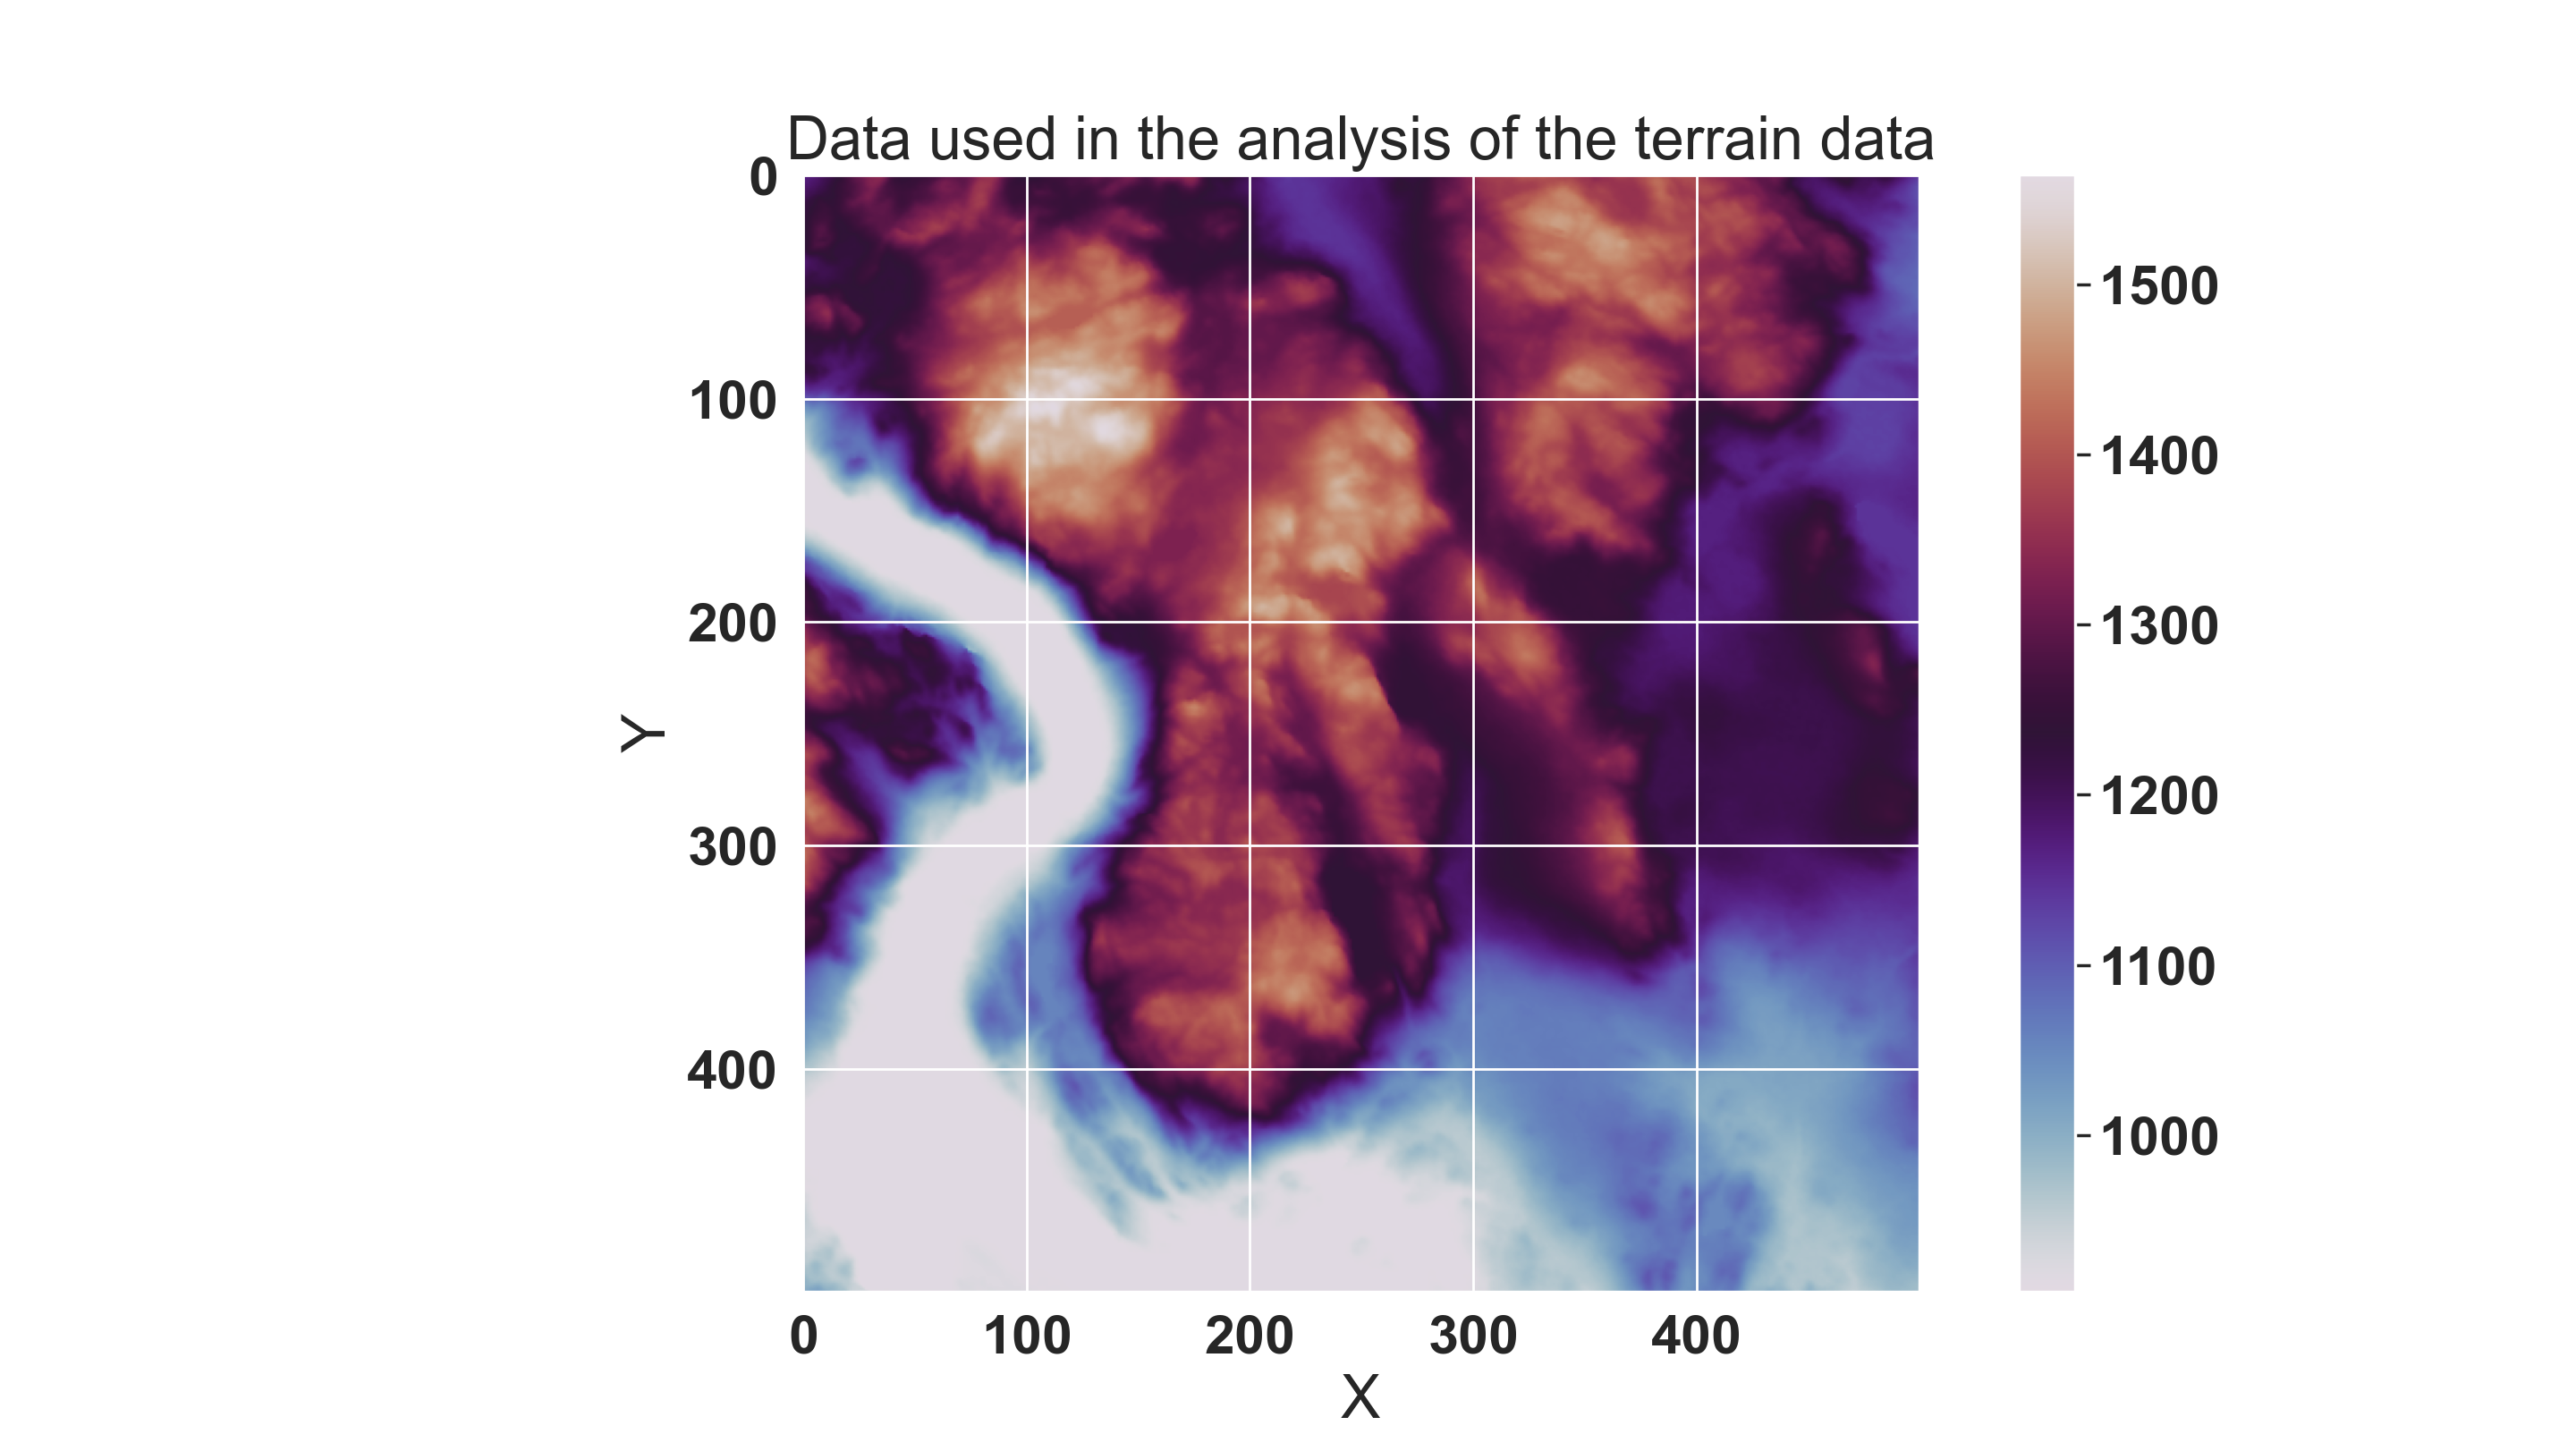
\includegraphics[width=\linewidth]{images/Figure_11.png}
	\caption{A plot of the data matrix used in the analysis of the terrain data in the second part of project 1.}
    \label{terrain_data}
\end{figure}
The data was also scaled by first subtracting the mean value from each column and then divide on the standard deviation so that the variation in height in our data set would not lead to huge MSE values. The OLS regression was applied to create a model of the data set fitted with polynomials of degree $0-10$. The same was done for Ridge, but here also a heat map of the MSE as a function of both different $\lambda$ values and complexity was created. The same was done for LASSO but here as mentioned above one had to downsize the data set to a $20 \cdot 20$ matrix when running over different $\lambda$ values, for the calculation of MSE and R2 score as a function of complexity the normal size data was used ($500 \cdot 500$ matrix).